%% Overleaf			
%% Software Manual and Technical Document Template	
%% 									
%% This provides an example of a software manual created in Overleaf.

\documentclass{../ol-softwaremanual}

% Packages used in this example
\usepackage{graphicx}  % for including images
\usepackage{microtype} % for typographical enhancements
\usepackage{minted}    % for code listings
\usepackage{amsmath}   % for equations and mathematics
\setminted{style=friendly,fontsize=\small}
\renewcommand{\listoflistingscaption}{List of Code Listings}
\usepackage{hyperref}  % for hyperlinks
\usepackage[a4paper,top=4.2cm,bottom=4.2cm,left=3.5cm,right=3.5cm]{geometry} % for setting page size and margins

\usepackage[english, greek]{babel}

\usepackage{subfig}

\usepackage{incgraph,tikz}

\usepackage{filemod}





\usepackage{rotating}


% Custom macros used in this example document
\newcommand{\doclink}[2]{\href{#1}{#2}\footnote{\url{#1}}}
\newcommand{\cs}[1]{\texttt{\textbackslash #1}}

\begin{document}
	
	
	\begin{titlepage}
		
		
		% Frontmatter data; appears on title page
		\title{\en Robustness Diagrams \\}
		\version{0.1}
		\softwarelogo{
\includegraphics[scale=0.4]{../CarBazaar_logo.png}}		
		
	\end{titlepage}
	
	
	\maketitle
	
	\newpage
	
	\center{\textbf{Μέλη Ομάδας}}
	
	\vspace{20pt}
	
	
	
	\begin{table}[htbp!]
		
		\begin{tabular}{llll}
			Μεμελετζόγλου Χαρίλαος & 1069364 & \en st1069364@ceid.upatras.gr & 4o Έτος   \\ 
			\\ Λέκκας Γεώργιος      &      1067430    &   \en st1067430@ceid.upatras.gr & 4o Έτος  \\
			\\ Γιαννουλάκης Ανδρέας        &   1067387       & \en st1067387@ceid.upatras.gr & 4o Έτος           \\
			\\ Κανελλόπουλος Ιωακείμ        &  1070914        &    \en st1070914@ceid.upatras.gr & 4o Έτος        \\ 
		\end{tabular}
	\end{table}
	
	\center{\textbf{Υπεύθυνοι Παρόντος Τεχνικού Κειμένου}}
	
	\vspace{20pt}
	
	\begin{table}[htbp!]
		\begin{tabular}{ll}
			Μεμελετζόγλου Χαρίλαος & \en Editor \\
			\\ Λέκκας Γεώργιος      &   \en  Editor \\
			\\ Γιαννουλάκης Ανδρέας & \en Contributor \\
			\\ Κανελλόπουλος Ιωακείμ & \en Contributor \\ 
		\end{tabular}
	\end{table}
	
	
	\vspace{20pt}
	
	\center{\textbf{Εργαλεία που χρησιμοποιήθηκαν}}
	
	\vspace{20pt}
	\flushleft
	Χρησιμοποιήθηκε το \en \doclink{https://www.overleaf.com/}{Overleaf} \gr και το \en \doclink{https://www.texstudio.org/}{TexStudio} \gr για την συγγραφή του \LaTeX\ κώδικα. \break
	
	Για την δημιουργία του λογότυπου, χρησιμοποιήθηκε το εργαλείο \en \doclink{https://www.adobe.com/express/create/logo}{Adobe Express} . \gr \break
	
	Για την δημιουργία των \en Robustness Diagrams \gr χρησιμοποιήθηκε το \en \doclink{https://www.visual-paradigm.com/}{Visual Paradigm} . \gr \break 
	
	\newpage
	
	\center{\textbf{\en Robustness Diagrams \gr}}
	\flushleft
	
	Οι εναλλακτικές ροές του κάθε \en Use Case \gr φαίνονται στο αντίστοιχο \en Robustness Diagram \gr, με κόκκινες ακμές και αντικείμενα. \break
	
	Για την ευκολότερη αντιστοίχιση ενός \en Use Case \gr στο αντίστοιχο \en Robustness Diagram \gr, παραθέτουμε και το κείμενο της κάθε Περίπτωσης Χρήσης, πρίν το διάγραμμα που προκύπτει. \\
	
	\newpage
	
	\paragraph{\en Use Case 1: \gr Ανάρτηση Αγγελίας Πώλησης Οχήματος}
	\centering
	
	\begin{enumerate}
		
		\item Ο χρήστης επιλέγει \en"\gr Ανάρτηση Αγγελίας Οχήματος\en" \gr στο αρχικού μενού
		\item Το σύστημα εμφανίζει την οθόνη Καταχώρησης Αγγελίας Πώλησης Οχήματος
		\item Ο χρήστης εισάγει την τοποθεσία του, τον τίτλο της αγγελίας, στοιχεία του οχήματος όπως μάρκα, μοντέλο, έτος κυκλοφορίας, χιλιόμετρα, κυβικά, τύπος καυσίμου, χρώμα, αριθμός πινακίδας, κλπ
		\item Το σύστημα ελέγχει πως όντως κυκλοφορεί αντίστοιχο μοντέλο αυτοκινήτου στην αγορά και εμφανίζει στον χρήστη την Οθόνη Ανάρτησης Εγγράφων Πιστοποίησης Κατάστασης Οχήματος
		\item Ο χρήστης ανεβάζει τα απαραίτητα έγγραφα που έχουν προκύψει από τον έλεγχο του οχήματος		
		\item Το σύστημα εμφανίζει στον χρήστη μια εκτίμηση της τιμής του οχήματος, με βάση την κατάστασή του
		\item Ο χρήστης επιλέγει να συνεχίσει με την προτεινόμενη τιμή ή εισάγει δικιά του
		\item Το σύστημα μεταφέρει τον χρήστη στην οθόνη Εισαγωγής Φωτογραφιών και Περιγραφής Οχήματος
		\item Ο χρήστης προσθέτει το κείμενο της περιγραφής και αναρτά τις φωτογραφίες του αυτοκινήτου
		\item Το σύστημα δημιουργεί το \en 3D \gr μοντέλο του οχήματος και εμφανίζει μια προεπισκόπηση της αγγελίας στον χρήστη
		\item Ο χρήστης εγκρίνει την αγγελία
		\item Το σύστημα δημιουργεί την αγγελία και εμφανίζει μήνυμα επιτυχούς ανάρτησης
	\end{enumerate}
	
	\paragraph{Εναλλακτική Ροή 1}
	
	\begin{enumerate}
		\item O χρήστης εισάγει στοιχεία μη-υπαρκτού μοντέλου
		\item Το σύστημα εμφανίζει προειδοποιητικό μήνυμα, επιστρέφει τον χρήστη στην οθόνη \textit{Καταχώρηση Αγγελίας Οχήματος}, προτρέποντάς τον να διορθώσει τα λανθασμένα πεδία
		\item Ο χρήστης προβαίνει στις απαραίτητες διορθώσεις και η Περίπτωση Χρήσης συνεχίζει από το βήμα 4 της βασικής ροής
	\end{enumerate}
	
	\paragraph{Εναλλακτική Ροή 2}
	
	\begin{enumerate}
		\item Ο χρήστης δεν εισάγει περιγραφή ή δεν αναρτά φωτογραφίες του οχήματος
		\item Το σύστημα εμφανίζει προειδοποιητικό μήνυμα, επιστρέφει τον χρήστη στην οθόνη \textit{Εισαγωγή Φωτογραφιών και Περιγραφής Οχήματος}, προτρέποντάς τον, να συμπληρώσει τα αντίστοιχα πεδία
		\item Ο χρήστης εισάγει τις απαραίτητες ελλείπουσες πληροφορίες και η Περίπτωση Χρήσης συνεχίζει από το βήμα 9 της βασικής ροής
	\end{enumerate}
	
	\paragraph{Εναλλακτική Ροή 3}
	
	\begin{enumerate}
		\item Ο χρήστης εισάγει τιμή η οποία είναι σημαντικά μεγαλύτερη από την προτεινόμενη από το σύστημα, τιμή
		\item Το σύστημα εμφανίζει προειδοποιητικό μήνυμα, επιστρέφει τον χρήστη στον οθόνη \textit{Εισαγωγή Τιμής}, προτρέποντάς τον, να εισάγει τιμή που δεν αποκλίνει τόσο από την προτεινόμενη τιμή
		\item Ο χρήστης επανεισάγει τιμή και η Περίπτωση Χρήσης συνεχίζει από το βήμα 8 της βασικής ροής
	\end{enumerate}

	\begin{figure}[htbp!]
		\includegraphics[scale=0.4]{img/rob\_post\_car\_listing.png}
		\caption{\en Robustness Diagram : "\gr Ανάρτηση Αγγελίας Πώλησης Οχήματος\en"\gr}
	\end{figure}
	


	
	\newpage
	
	
	\paragraph{\en Use Case 2: \gr Προγραμματισμός Ελέγχου Οχήματος}
	
	\begin{enumerate}
		\item Ο χρήστης επιλέγει \en"\gr Έλεγχος Οχήματος\en" \gr στο αρχικό μενού
		\item Το σύστημα εμφανίζει την σελίδα Προγραμματισμού Ελέγχου Οχήματος
		\item Ο χρήστης επιλέγει το πακέτο ελέγχου που επιθυμεί, αν επιθυμεί την έκδοση πιστοποιητικών εγγράφων της κατάστασης του οχήματος, την ημερομηνία και ώρα διεξαγωγής του ελέγχου και εισάγει την τοποθεσία του
		\item Το σύστημα αφού επιβεβαιώσει την εισαχθείσα τοποθεσία, προτείνει στην χρήστη έναν ελεγκτή, με βάση την τοποθεσία που εισήγαγε
		\item Ο χρήστης αποδέχεται ή όχι τον προτεινόμενο ελεγκτή
		\item Το σύστημα εμφανίζει την οθόνη Εισαγωγή Κωδικού Αγγελίας, στο όχημα της οποίας θα πραγματοποιηθεί ο έλεγχος		
		\item Ο χρήστης εισάγει τον κωδικό της αγγελίας
		\item Το σύστημα ανακτά τα στοιχεία του οχήματος από την αγγελία και εμφανίζει την τελική τιμή του ελέγχου καθώς και την χρονική διάρκειά του
		\item Ο χρήστης επιβεβαιώνει τα στοιχεία
		\item Το σύστημα μεταφέρει τον χρήστη στο μενού πληρωμών. Μετά την επιτυχή πληρωμή, γίνεται καταχώρηση της συναλλαγής στο \en \textit{TransactionLog} \gr, το σύστημα εμφανίζει μήνυμα επιτυχούς κράτησης και αποστέλλει \en email \gr στον χρήστη, με τα στοιχεία του ραντεβού και του ελεγκτή		
	\end{enumerate}
	
	\paragraph{Εναλλακτική Ροή 1}
	
	\begin{enumerate}
		\item Ο χρήστης εισάγει μη-υπαρκτή τοποθεσία
		\item Το σύστημα ενημερώνει τον χρήστη με το κατάλληλο μήνυμα σφάλματος 
		\item Ο χρήστης εισάγει την σωστή τοποθεσία του
		\item Το σύστημα εντοπίζει τον χρήστη και η Περίπτωση Χρήσης προχωρά από το βήμα 4 της βασικής ροής
	\end{enumerate}
	
	\paragraph{Εναλλακτική Ροή 2}
	
	\begin{enumerate}
			\item Ο χρήστης απορρίπτει τον προτεινόμενο από το σύστημα ελεγκτή, προκειμένου να επιλέξει τον ελεγκτή της αρεσκείας του
			\item Το σύστημα εμφανίζει την οθόνη εισαγωγής στοιχείων του ελεγκτή
			\item Ο χρήστης εισάγει τα στοιχεία του ελεγκτή
			\item Το σύστημα ελέγχει πως υπάρχει πράγματι εγγεγραμμένος ο εν λόγω ελεγκτής και αν ναι, η Περίπτωση Χρήσης συνεχίζει από το βήμα 6 της βασικής ροής. Ειδάλλως, εμφανίζει μήνυμα σφάλματος και ο έλεγχος ακυρώνεται	
	\end{enumerate}	


	\begin{figure}[htbp!]
		\includegraphics[scale=0.45]{img/rob\_car\_check.png}
		\caption{\en Robustness Diagram : "\gr Προγραμματισμός Ελέγχου Οχήματος\en"\gr}
	\end{figure}
	
	
	\newpage
	\centering
	
	\paragraph{\en Use Case 3: \gr Αναζήτηση Ανταλλακτικού}	
	
	\begin{enumerate}
		\item Ο χρήστης επιλέγει \en"\gr Αναζήτηση Ανταλλακτικού\en" \gr στο αρχικό μενού
		\item Το σύστημα εμφανίζει την οθόνη Εισαγωγή Χαρακτηριστικών Ανταλλακτικού
		\item Ο χρήστης περιορίζει την αναζήτηση του τοποθετώντας το είδος του οχήματος, την μάρκα, το μοντέλο, τον κατασκευαστή, το εύρος τιμών, και την κατάσταση του ανταλλακτικού (καινούργιο ή μεταχειρισμένο) 
		\item Το σύστημα εμφανίζει την οθόνη Αποτελέσματα Αναζήτησης, με την λίστα με τις αγγελίες ανταλλακτικών που πληρούν τα κριτήρια που έθεσε ο χρήστης
		\item Ο χρήστης επιλέγει την αγγελία της αρεσκείας του
		\item Το σύστημα μεταφέρει τον χρήστη στην οθόνη Αγγελία Ανταλλακτικού, εμφανίζοντας μια λεπτομερή περιγραφή του ανταλλακτικού και τα στοιχεία του πωλητή
		
	\end{enumerate}
	
	\paragraph{Εναλλακτική Ροή}
	
	\begin{enumerate}
		\item Ο χρήστης δεν εισάγει χαρακτηριστικά για το ανταλλακτικό που επιθυμεί να αγοράσει
		\item Το σύστημα του εμφανίζει ανταλλακτικά για όλες τις κατηγορίες και μάρκες αυτοκινήτων και προχωρά από το βήμα 4 της βασικής ροής
	\end{enumerate}

	
	\begin{figure}[htbp!]
		\includegraphics[scale=0.6]{img/rob\_spare\_part\_search.png}
		\caption{\en Robustness Diagram : "\gr Αναζήτηση Ανταλλακτικού\en"\gr}
	\end{figure}




	
	\newpage
	
	\centering
	\paragraph{\en Use Case 5: \gr Σύγκριση Αυτοκινήτων}
	\begin{enumerate}
		\item Ο χρήστης επιλέγει \en"\gr Σύγκριση Αυτοκινήτων\en" \gr στο αρχικό μενού
		\item Το σύστημα εμφανίζει την οθόνη Σύγκρισης Αυτοκινήτων και προτρέπει τον χρήστη να εισάγει τους κωδικούς διαφορετικών αγγελιών, τα οχήματα των οποίων επιθυμεί να συγκρίνει
		\item Ο χρήστης εισάγει τους κωδικούς των αγγελιών
		\item Το σύστημα ελέγχει αν εισήχθησαν κωδικοί και αν είναι διαφορετικοί μεταξύ τους. Στην συνέχεια, εμφανίζει την οθόνη Κριτήρια Αυτοκινήτων προς Σύγκριση, προτρέποντας τον χρήστη να εισάγει το επιθυμητό εύρος τιμών και τα σημαντικά κριτήρια που θα συντελέσουν στην επιλογή ενός οχήματος
		\item Ο χρήστης εισάγει το επιθυμητό εύρος τιμών και καθορίζει τα κυρίαρχα κριτήρια της σύγκρισης
		\item Το σύστημα εμφανίζει την οθόνη Αποτελέσματα Αναζήτησης, προβάλλοντας μία λίστα με τα αυτοκίνητα και τα χαρακτηριστικά που ο χρήστης επέλεξε να πάρουν μέρος στην σύγκριση, αλλά και το κόστος των τελών κυκλοφορίας και των ασφαλίστρων. Επίσης, το σύστημα προτείνει στον χρήστη κατάλληλα οχήματα με βάση τα κριτήρια σύγκρισης
		\item Ο χρήστης επιλέγει το όχημα που επιθυμεί
		\item Το σύστημα μεταφέρει τον χρήστη στην οθόνη Λεπτομέρειες Αγγελίας, επιτρέποντάς του να εξετάσει αναλυτικότερα το επιλεγμένο όχημα
	\end{enumerate}
	
	\paragraph{Εναλλακτική Ροή 1}
	
	\begin{enumerate}
		\item Ο χρήστης δεν εισάγει κωδικούς αγγελιών \red{ή οι κωδικοί που εισήγαγε δεν είναι διαφορετικοί μεταξύ τους}
		\item Το σύστημα εμφανίζει προειδοποιητικό μήνυμα και προτείνει στον χρήστη παρόμοια οχήματα με αυτά που έχει αποθηκεύσει στην \en wishlist \gr του αλλά και οχήματα που συμμετέχουν συχνά σε συγκρίσεις άλλων χρηστών
		\item Ο χρήστης καθορίζει τα κριτήρια σύγκρισης και η Περίπτωση Χρήσης συνεχίζει από το βήμα 5 της βασικής ροής
	\end{enumerate}
	
	\begin{figure}[htbp!]
		\includegraphics[scale=0.45]{img/rob\_vehicle\_compare.png}
		\caption{\en Robustness Diagram : "\gr Σύγκριση Αυτοκινήτων\en"\gr}
	\end{figure}

	\newpage
	\centering
	
	\paragraph{\en Use Case 6: \gr Προσθήκη Καταστήματος Αντιπροσωπείας}
	
	\begin{enumerate}
		\item Ο υπεύθυνος της αντιπροσωπείας επιλέγει \en"\gr Προσθήκη Καταστήματος\en" \gr στο αρχικό μενού
		\red{\item Το σύστημα εμφανίζει την οθόνη Εισαγωγής Καταστήματος Αντιπροσωπείας, προτρέποντας τον χρήστη να εισάγει το όνομα της εταιρείας στην οποία υπάγεται η αντιπροσωπεία}
		\item Ο υπεύθυνος εισάγει το όνομα της εταιρείας
		\item Το σύστημα επιβεβαιώνει πως στην Βάση Δεδομένων της πλατφόρμας, υπάρχει εγγεγραμμένη η αντίστοιχη εταιρεία και στην συνέχεια, εμφανίζει τον χάρτη και ζητά από τον χρήστη να εισάγει την τοποθεσία του καταστήματος
		\item Ο υπεύθυνος της αντιπροσωπείας εισάγει τα λεπτομερή γεωγραφικά στοιχεία του καταστήματος
		\item Το σύστημα εντοπίζει το κατάστημα στον χάρτη και εμφανίζει την οθόνη Λεπτομέρειες Καταστήματος, ζητώντας από τον χρήστη να εισάγει τον τίτλο του καταστήματος και μια λίστα με τα αυτοκίνητα που διαθέτει προς πώληση
		\item Ο υπεύθυνος εισάγει τον τίτλο και τα οχήματα που διαθέτει το κατάστημα
		\red{\item Το σύστημα μεταφέρει τον χρήστη στην οθόνη Επιβεβαίωσης, στην οποία εμφανίζονται τα στοιχεία του καταστήματος (όνομα, τοποθεσία) και η λίστα με τα αυτοκίνητα που διαθέτει}
		\red{\item Ο υπεύθυνος επιβεβαιώνει τα στοιχεία		}
		\item Το σύστημα εμφανίζει την οθόνη Δημιουργία Διαφήμισης, προτρέποντας τον χρήστη, να δημιουργήσει μια διαφήμιση για το συγκεκριμένο κατάστημα, με σκοπό την ενημέρωση των χρηστών της πλατφόρμας που βρίσκονται στην περιοχή του καταστήματος
		\item Ο υπεύθυνος δημιουργεί την σχετική διαφήμιση
		\red{\item Το σύστημα δημιουργεί την διαφήμιση, καταχωρεί το κατάστημα και εμφανίζει μήνυμα επιτυχούς προσθήκης καταστήματος}
	\end{enumerate}
	
	\paragraph{Εναλλακτική Ροή 1}
	
	\begin{enumerate}
		\item Ο υπεύθυνος της αντιπροσωπείας εισάγει όνομα εταιρείας, η οποία δεν ανήκει στην πλατφόρμα
		\red{\item Το σύστημα εμφανίζει προειδοποιητικό μήνυμα και μεταφέρει τον χρήστη στην οθόνη Εγγραφή Εταιρείας, προτρέποντας τον χρήστη να εγγράψει στην πλατφόρμα την εταιρεία με το όνομα που εισήγαγε		}
		\item Ο υπεύθυνος εγγράφει την εταιρεία εισάγοντας τα απαραίτητα στοιχεία
		\red{\item Το σύστημα καταχωρεί την εταιρεία στις ήδη εγγεγραμμένες και η Περίπτωση Χρήσης συνεχίζει από το βήμα 4 της βασικής ροής}
	\end{enumerate}

	\begin{figure}[htbp!]
		\includegraphics[scale=0.50]{img/rob\_add\_dealership\_store.png}
		\caption{\en Robustness Diagram : "\gr Προσθήκη Καταστήματος Αντιπροσωπείας}
	\end{figure}
	
	
	\newpage
	\centering
	\paragraph{\en Use Case 7: \gr Προγραμματισμός \en Test Drive \gr}
	
	\begin{enumerate}
		\item Ο χρήστης επιλέγει \en"Test Drive" \gr στο αρχικό μενού
		\item Το σύστημα εμφανίζει την οθόνη οθόνη Καταχώρησης Κωδικού Αγγελίας Οχήματος
		\item Ο χρήστης εισάγει τον κωδικό της αγγελίας, για το όχημα της οποίας ενδιαφέρεται για \en Test Drive \gr
		\item Το σύστημα ελέγχει πως ο κωδικός αντιστοιχεί σε καταχωρημένη αγγελία και μεταφέρει τον χρήστη στην οθόνη Προγραμματισμού \en Test Drive \gr
		\item Ο χρήστης εισάγει την επιθυμητή ημερομηνία και ώρα
		\item Το σύστημα εμφανίζει τα στοιχεία του ραντεβού
		\item Ο χρήστης επιβεβαιώνει τα στοιχεία
		\item Το σύστημα εμφανίζει την οθόνη Επιτυχούς προγραμματισμού \en Test Drive \gr και αποστέλλει στο \en email \gr του χρήστη και του πωλητή του οχήματος, τα λεπτομερή στοιχεία του ραντεβού 
	\end{enumerate}
	
	\paragraph{Εναλλακτική Ροή 1}
	
	\begin{enumerate}
		\item Ο χρήστης επιλέγει μη-διαθέσιμη ημερομηνία και ώρα
		\item Το σύστημα εμφανίζει μήνυμα σφάλματος σχετικά με την μη-διαθεσιμότητα της επιλεγμένης ημερομηνίας και μεταφέρει τον χρήστη στην οθόνη \textit{Προγραμματισμού \en Test Drive \gr}, προτρέποντάς τον επιλέξει ξανά
		\item Ο χρήστης επιλέγει νέα ημερομηνία και ώρα και η Περίπτωση Χρήσης συνεχίζει από το βήμα 6 της βασικής ροής
	\end{enumerate}
	
	
	\paragraph{\red{Εναλλακτική Ροή 2}}
	
	\red{\begin{enumerate}
			\item Ο χρήστης εισάγει κωδικό μη-καταχωρημένης αγγελίας
			\item Το σύστημα εμφανίζει σχετικό μήνυμα σφάλματος και μεταφέρει τον χρήστη στην οθόνη \textit{Καταχώρησης Κωδικού Αγγελίας Οχήματος}, προτρέποντάς τον να επανεισάγει τον κωδικό
			\item Ο χρήστης εισάγει τον κωδικό της αγγελίας και η Περίπτωση Χρήσης συνεχίζει από το βήμα 4 της βασικής ροής
	\end{enumerate}}

	\begin{figure}[htbp!]
		\includegraphics[scale=0.35]{img/rob\_test\_drive.png}
		\caption{\en Robustness Diagram : "\gr Προγραμματισμός \en Test Drive"\gr}
	\end{figure}
	
	\newpage
	\centering
	
		\paragraph{\en Use Case 9: \gr Αγορά Οχήματος\gr}
	
	\begin{enumerate}
		\item Ο χρήστης επιλέγει \en"\gr Αγορά Οχήματος\en" \gr στο αρχικό μενού
		\item Το σύστημα αποστέλλει έναν κωδικό ασφαλείας στο \en email \gr του χρήστη και εμφανίζει την οθόνη Εισαγωγής Κωδικού Ασφαλείας
		\item Ο χρήστης εισάγει τον κωδικό ασφαλείας		
		\item Το σύστημα εμφανίζει την οθόνη Εισαγωγής Κωδικού Αγγελίας Οχήματος
		\item Ο χρήστης εισάγει τον κωδικό της αγγελίας	του οχήματος που επιθυμεί να αγοράσει
		\item Το σύστημα ελέγχει πως ο δοσμένος κωδικός αντιστοιχεί σε καταχωρημένη αγγελία και ανακτά τα στοιχεία του οχήματος. Στην συνέχεια, μεταφέρει τον χρήστη στην οθόνη Διαχείριση Οικονομικών, ρωτώντας τον χρήστη αν επιθυμεί να πληρώσει με άτοκες δόσεις. Σε περίπτωση που ο χρήστης επιλέξει την πληρωμή με δόσεις, το σύστημα εμφανίζει την οθόνη της υπηρεσίας \en"\gr Οικονομικός Σύμβουλος\en"\gr
		\item Ο χρήστης επιλέγει να πληρώσει με άτοκες δόσεις
		\item Το σύστημα εμφανίζει την οθόνη του Οικονομικού Συμβούλου και ζητά από τον χρήστη να εισάγει τον μηνιαίο μισθό του, με σκοπό τον υπολογισμό ενός προσαρμοσμένου στον χρήστη, ποσού άτοκης μηνιαίας δόσης
		\item Ο χρήστης εισάγει τον μηνιαίο μισθό του
		\item Το σύστημα εμφανίζει το υπολογισμένο ποσό μηνιαίας δόσης, καθώς και το κόστος των τελών κυκλοφορίας του οχήματος
		\item Ο χρήστης αποδέχεται το ποσό της μηνιαίας δόσης
		\item Το σύστημα εμφανίζει την οθόνη Ολοκλήρωσης Αγοράς, με την τιμή του οχήματος, τον κωδικό της αγγελίας, το όνομα του οχήματος και το ποσό της μηνιαίας δόσης σε περίπτωση που η πληρωμή θα γίνει μέσω άτοκων δόσεων. Στην συνέχεια, το σύστημα μεταφέρει τον χρήστη στην σελίδα του συστήματος πληρωμών
		\item Ο χρήστης πληρώνει για την αγορά του οχήματος
		\item Το σύστημα καταχωρεί την συναλλαγή στο \en \textit{TransactionLog} \gr, εμφανίζει μήνυμα επιτυχούς αγοράς και αποστέλλει στο \en email \gr του χρήστη την απόδειξη πληρωμής καθώς και τον κωδικό της συναλλαγής
	\end{enumerate}
	
	\paragraph{Εναλλακτική Ροή 1}
	\begin{enumerate}
		\item Ο χρήστης επιλέγει να μην πληρώσει με άτοκες δόσεις και η Περίπτωση Χρήσης συνεχίζει από το βήμα 12 της βασικής ροής
	\end{enumerate}
	
	\paragraph{Εναλλακτική Ροή 2}
	\begin{enumerate}
		\item Ο χρήστης εισάγει κωδικό μη-υπαρκτής αγγελίας
		\item Το σύστημα εμφανίζει μήνυμα μη-υπαρκτής αγγελίας και επιστρέφει τον χρήστη στην οθόνη \textit{Εισαγωγή Κωδικού Αγγελίας Οχήματος} 
		\item Ο χρήστης επανεισάγει κωδικό και η Περίπτωση Χρήσης συνεχίζει από το βήμα 6 της βασικής ροής
	\end{enumerate}

	\begin{figure}[htbp!]
		\includegraphics[scale=0.33]{img/rob\_purchase\_car.png}
		\caption{\en Robustness Diagram : "\gr Αγορά Οχήματος\en"\gr}
	\end{figure}


	
	\newpage
	
	\centering
	\paragraph{\en Use Case 12: \gr Ανάρτηση Αγγελίας Πώλησης Ανταλλακτικού \gr}
	
	\begin{enumerate}
		\item Ο χρήστης επιλέγει \en"\gr Ανάρτηση Αγγελίας Ανταλλακτικού\en" \gr στο αρχικό μενού
		\item Το σύστημα εμφανίζει την οθόνη Ανάρτησης Αγγελίας Ανταλλακτικού
		\item Ο χρήστης εισάγει την τοποθεσία του και τον τίτλο της αγγελίας
		\item Το σύστημα εμφανίζει την οθόνη Εισαγωγή στοιχείων Ανταλλακτικού
		\item Ο χρήστης εισάγει στοιχεία του ανταλλακτικού όπως η κατάστασή του (καινούριο ή μεταχειρισμένο), τον τύπο του, τον κωδικό του, την εταιρεία, το μοντέλο και την τιμή του
		\item Το σύστημα ελέγχει πως όντως υπάρχει ανταλλακτικό με τον δοσμένο κωδικό και εμφανίζει την οθόνη Εισαγωγής Φωτογραφιών και Περιγραφής Ανταλλακτικού
		\item Ο χρήστης προσθέτει το κείμενο της περιγραφής και αναρτά τις φωτογραφίες του ανταλλακτικού
		\item Το σύστημα ελέγχει πως προστέθηκε περιγραφή και αναρτήθηκαν φωτογραφίες.
		\item Το σύστημα δημιουργεί την αγγελία, καταχωρεί το κύριο ανταλλακτικό στην κατάλληλη κατηγορία με βάση τον κωδικό του και εμφανίζει μια προεπισκόπηση της αγγελίας
		\item Ο χρήστης εγκρίνει την αγγελία
		\item Το σύστημα καταχωρεί την αγγελία και εμφανίζει μήνυμα επιτυχούς ανάρτησης
	\end{enumerate}
	
	
	\paragraph{Εναλλακτική Ροή 1}
	
	\begin{enumerate}
		\item Ο χρήστης εισάγει κωδικό μη-υπαρκτού ανταλλακτικού
		\item Το σύστημα εμφανίζει προειδοποιητικό μήνυμα και επιστρέφει τον χρήστη στην Οθόνη \textit{Εισαγωγή στοιχείων Ανταλλακτικού}
		\item Ο χρήστης επανεισάγει τον κωδικό και η Περίπτωση Χρήσης προχωρά από το βήμα 5 της βασικής ροής
	\end{enumerate}
	
	\paragraph{\red{Εναλλακτική Ροή 2}}
	
	\red{\begin{enumerate}
			\item Ο χρήστης δεν εισάγει περιγραφή ή δεν αναρτά φωτογραφίες του ανταλλακτικού
			\item Το σύστημα εμφανίζει προειδοποιητικό μήνυμα, και επιστρέφει τον χρήστη στην οθόνη \textit{Εισαγωγή Φωτογραφιών και Περιγραφής Ανταλλακτικού}, προτρέποντάς τον να συμπληρώσει τα αντίστοιχα πεδία
			\item Ο χρήστης εισάγει τις απαραίτητες ελλείπουσες πληροφορίες και η Περίπτωση Χρήσης συνεχίζει από το βήμα 8 της βασικής ροής
	\end{enumerate}}
	
	\begin{figure}[htbp!]
		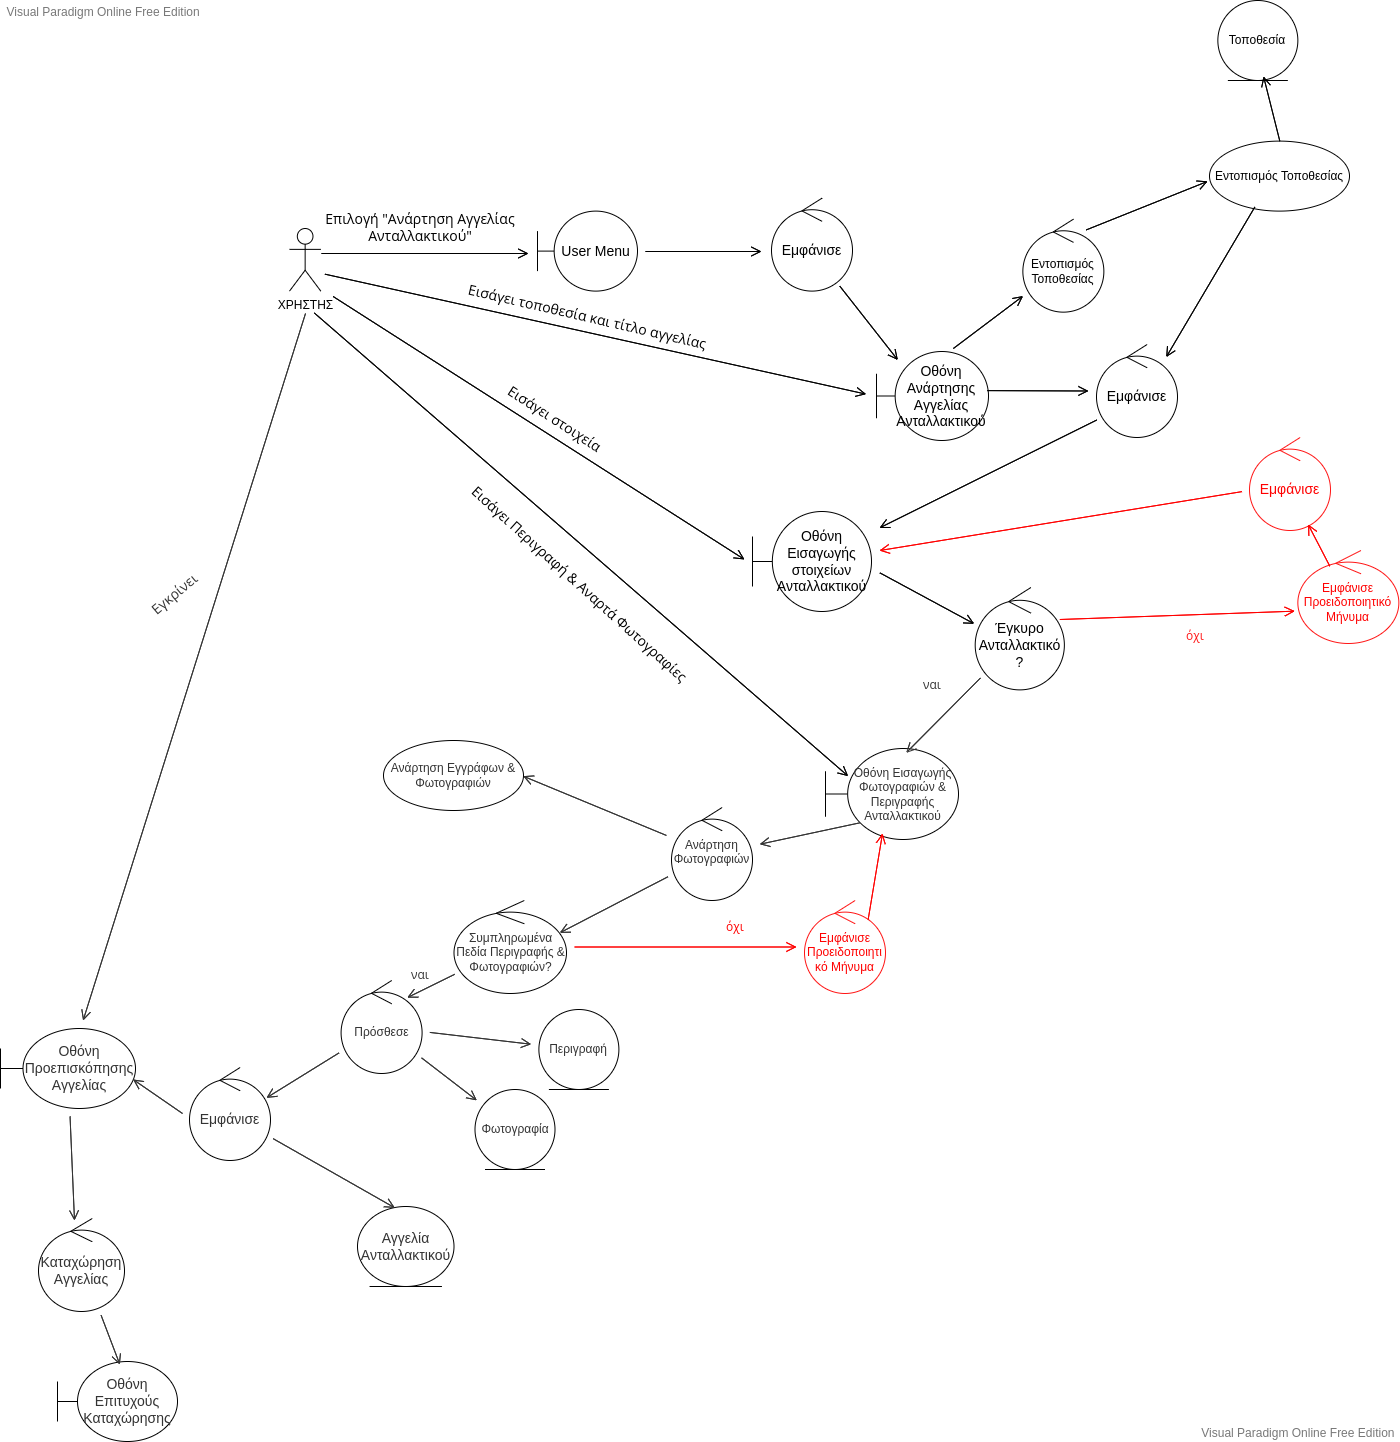
\includegraphics[scale=0.35]{img/rob_spare_part_listing.png}
		\caption{\en Robustness Diagram : "\gr Ανάρτηση Αγγελίας Πώλησης Ανταλλακτικού\en"\gr}
	\end{figure}

	\newpage
	\centering
	
	\paragraph{\en Use Case 13: \gr Έλεγχος Αναφοράς}  
	\begin{enumerate}
		\item Ο υπάλληλος της Ασφαλιστικής εταιρείας επιλέγει \en"\gr Έλεγχος αναφοράς\en" \gr στο αρχικό μενού
		\item Το σύστημα εμφανίζει την οθόνη Καταχωρημένες Αναφορές, η οποία περιέχει την λίστα με τις αναφορές, τον κωδικό τους και την κατάστασή τους (\en"\gr σε εκκρεμότητα \en" \gr κλπ)
		\item Ο υπάλληλος επιλέγει ή εισάγει τον κωδικό της αναφοράς που επιθυμεί να ελέγξει 
		\item Το σύστημα μεταφέρει τον χρήστη στην οθόνη Λεπτομέρειες Αναφοράς, εμφανίζοντας την αγγελία και την λίστα με τις αναφορές που έχει λάβει, καθώς και στοιχεία αυτών όπως τον δημιουργό, την ημερομηνία υποβολής και την αιτία αναφοράς 
		\item Ο υπάλληλος της εταιρείας, εξετάζει την αγγελία μαζί με την αναφορά και  επιλέγει να διαγράψει την αγγελία ενημερώνοντας και τον δημιουργό της αναφοράς αλλά και τον δημιουργό της αγγελίας. 
		\item To σύστημα διαγράφει την αναφορά μαζί με την αγγελία
	\end{enumerate}
	
	\paragraph{Εναλλακτική Ροή 1}
	\begin{enumerate}
		\item Ο υπάλληλος της ασφαλιστικής εταιρείας εισάγει κωδικό αναφοράς που δεν αντιστοιχεί σε κάποια καταχωρημένη αναφορά
		\item Το σύστημα εμφανίζει προειδοποιητικό μήνυμα και τον μεταφέρει στην οθόνη \textit{Καταχωρημένες Αναφορές}, προτρέποντάς τον εισάγει ξανά τον κωδικό ή να επιλέξει μια αναφορά και η Περίπτωση Χρήσης συνεχίζει από το βήμα 3 της βασικής ροής		
	\end{enumerate}	
	
	\begin{figure}[htbp!]
		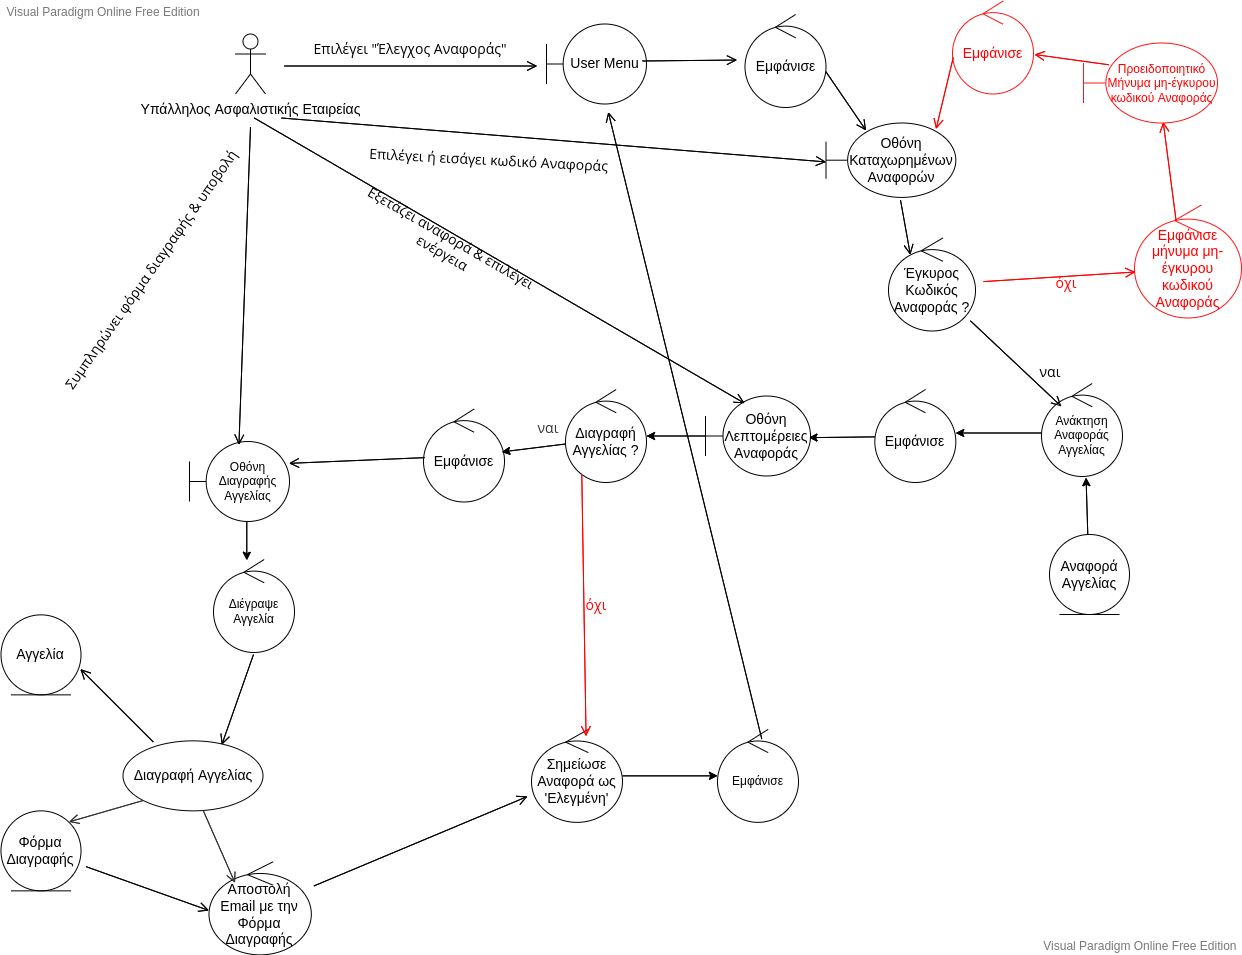
\includegraphics[scale=0.41]{img/rob_check_report.png}
		\caption{\en Robustness Diagram : "\gr Έλεγχος Αναφοράς\en"\gr}
	\end{figure}

	\newpage
	\centering
	
	\paragraph{\en Use Case 14: \gr Αγορά Ασφαλιστικού Πακέτου}
	\begin{enumerate}
		\item Ο χρήστης επιλέγει \en"\gr Αγορά Ασφαλιστικού Πακέτου\en" \gr στο αρχικό μενού
		\item Το σύστημα εμφανίζει την οθόνη Εισαγωγής Κωδικού Συναλλαγής
		\item Ο χρήστης εισάγει τον κωδικό της συναλλαγής, για το όχημα της οποίας επιθυμεί να αγοράσει ασφαλιστική κάλυψη
		\item Το σύστημα μεταφέρει τον χρήστη στην οθόνη Επιλογής Ασφαλιστικού Πακέτου, στην οποία εμφανίζονται τα στοιχεία της αγοράς του οχήματος. Το σύστημα προτρέπει τον χρήστη να επιλέξει το ασφαλιστικό πακέτο που επιθυμεί. Επίσης, ρωτά τον χρήστη, αν επιθυμεί να εξαργυρώσει πόντους που κατέχει, με σκοπό την εξασφάλιση έκπτωσης στα ασφάλιστρα
		\item Ο χρήστης επιλέγει ασφαλιστικό πακέτο και σε περίπτωση που επιθυμεί να εξαργυρώσει πόντους, εισάγει το επιθυμητό ποσό
		\item Το σύστημα υπολογίζει και εμφανίζει την οθόνη Τιμή Ασφαλίστρων, όπου περιέχεται η τελική τιμή και στην συνέχεια μεταφέρει τον χρήστη στο μενού πληρωμών
		\item Ο χρήστης αποδέχεται τα ασφάλιστρα
		\item Το σύστημα δημιουργεί το Ασφαλιστικό Συμβόλαιο και μεταφέρει τον χρήστη στην οθόνη του συστήματος πληρωμών. Μετά την ολοκλήρωση της πληρωμής, το σύστημα καταγράφει την συναλλαγή στο \en \textit{TransactionLog} \gr και αποστέλλει \en email \gr στον χρήστη, με το Συμβόλαιο του Ασφαλιστικού Πακέτου και την Απόδειξη Συναλλαγής. Τέλος, εμφανίζει μήνυμα επιτυχούς αγοράς.		
	\end{enumerate}
	
	\paragraph{Εναλλακτική Ροή }
	
	 \begin{enumerate}
			\item Ο χρήστης εισάγει κωδικό μη-καταγεγραμμένης συναλλαγής
			\item Το σύστημα ειδοποιεί τον χρήστη και τον προτρέπει να ελέγξει τον κωδικό που εισήγαγε
			\item Ο χρήστης επανεισάγει τον κωδικό και η Περίπτωση Χρήσης συνεχίζει από το βήμα 4 της βασικής ροής
	\end{enumerate}

	\begin{figure}[htbp!]
		\includegraphics[scale=0.48]{img/rob\_purchase\_insurance\_plan.png}
		\caption{\en Robustness Diagram : "\gr Αγορά Ασφαλιστικού Πακέτου\en"\gr}
	\end{figure}
	
	
	
	
	
	
	
	
	
	
	
\end{document}



 
